\documentclass[14pt]{article}

\usepackage[polish]{babel}
\usepackage[utf8]{inputenc}
\usepackage[T1]{fontenc}
\usepackage{extsizes}
\usepackage{graphicx}
\usepackage{tocloft}
\usepackage{amsmath}
\usepackage{multirow}
\usepackage{hyperref}


\font\titlefont=cmtt10 at 22pt

\title{
    
\includegraphics[scale=0.5]{images/logo-pwr-pion.png}
    \vspace{1cm}
    \\
    {\textbf{
    \titlefont Sygnały i obrazy cyfrowe
    \\ Laboratorium 1 - Aliasing 2D
    }}
}
    
\author{
    Informatyczne Systemy Automatyki
    \\
    \\ Wykonujący:
    \\ Igor Potyrała - 272518
    %\\ Antoni Kirylczuk - 272556
    \\
    \\ Prowadzący - Przemysław Śliwiński
}
\date{Data laboratoriów: 11 października 2023}


\begin{document}
\maketitle
\newpage
% Spis treści
%\newpage
%\renewcommand{\cftsecleader}{\cftdotfill{\cftdotsep}}
%{
 % \hypersetup{linkcolor=black, hidelinks}
 % \tableofcontents
%}

% Wstęp teoretyczny, definicje
\section{Zadania}
\subsection{Sekwencja obrazów}
Celem zadania pierwszego było wygenerowanie sekwencjii
$M = 64$ obrazów przedstawiających kręcacę się śmigło, z $n = 3$,
5 łopatkami. Wykonać to można byłO za pomocą współrzędnych
biegunowych oraz funkcji:
\begin{center}
    $f(x) = \sin(nx + \frac{m \pi}{RPM})$\
    \vspace{0.5cm}
    \\ $m$ - aktualna klatka, gdzie $m \subset <-32;32>$
    \\ $RPM$ - liczba obrotów na minute, u nas  $RPM=10$
    \\ $x$ - wartość X współrzędnych biegunowych
    \\ $n$ - liczba łopatek

    \vspace{1cm}
    \begin{minipage}{7cm}
        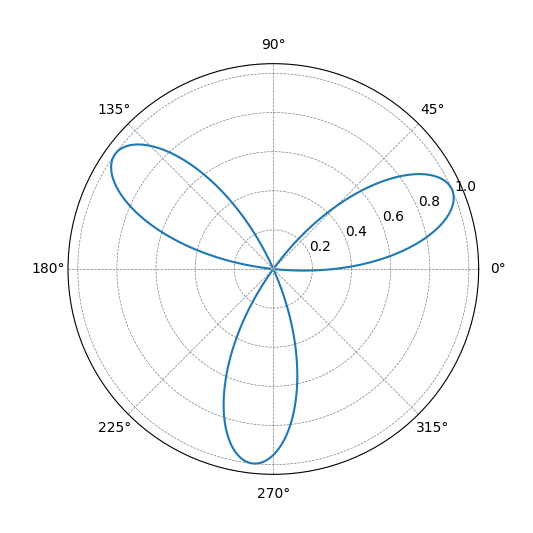
\includegraphics[scale=0.5]{images/propeller_3.png}
        \\ \small Obraz 1. Kręcacę się śmigło z $n = 3$ łopatkami.
    \end{minipage}
    \hfill
    \begin{minipage}{7cm}
        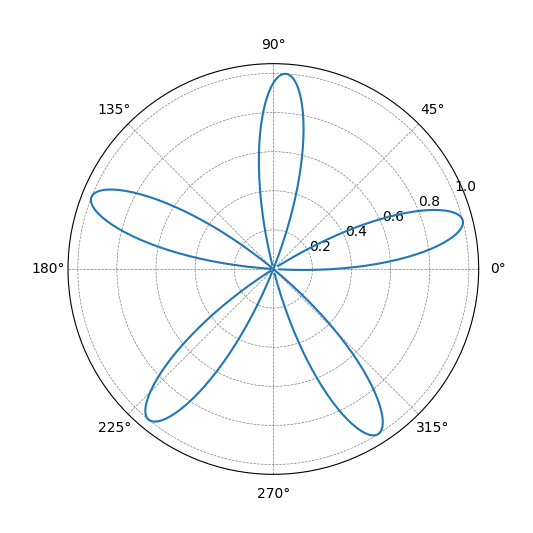
\includegraphics[scale=0.5]{images/propeller_5.png}
        \\ \small Obraz 2. Kręcacę się śmigło z $n = 5$ łopatkami.
    \end{minipage}
\end{center}

\newpage
Następnie by wygenerować kręcacę się śmigło skorzystamy z funkcji
FuncAnimation oraz PillowWriter biblioteki matplotlib.
\begin{center}
    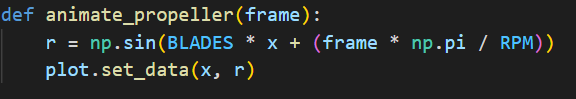
\includegraphics[scale=0.53]{images/animate.png}
    \\ \small Kod 1. Generacja obrazu śmigła.

    \vspace{0.25cm}
    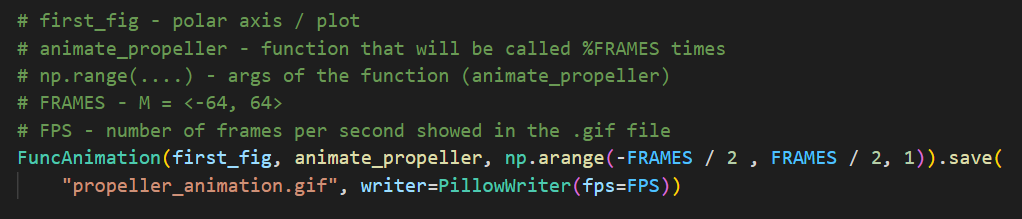
\includegraphics[scale=0.3]{images/func_anim.png}
    \\ \small Kod 2. Animacja obrazu.
\end{center}



%
\subsection{Sensor}
Drugie zadanie wymagało sprawdzenia szybkości sensora mającego
rozdzielczość 256 x 256 pikseli. Sensor był w stanie odczytać 
l = 1, ... , 16 linii. Następnie należało utworzyć film 
uruchamiający sekwencję obrazów "w kółko". 
Można było tego dokonać robiąc zrzuty ekranu i
wklejając je po kolei od góry obrazu zależnie od 
zmiennej l = 1, ..., 16.

\begin{center}
    \vspace{0.5cm}
    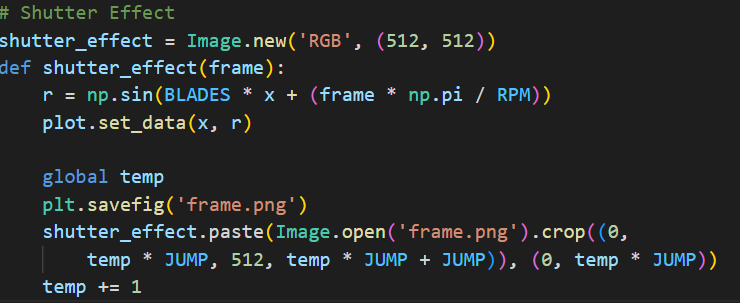
\includegraphics[scale=0.55]{images/shutter.png}
    \\ \small Kod 3. Funkcja imitująca sensor.

    \newpage
    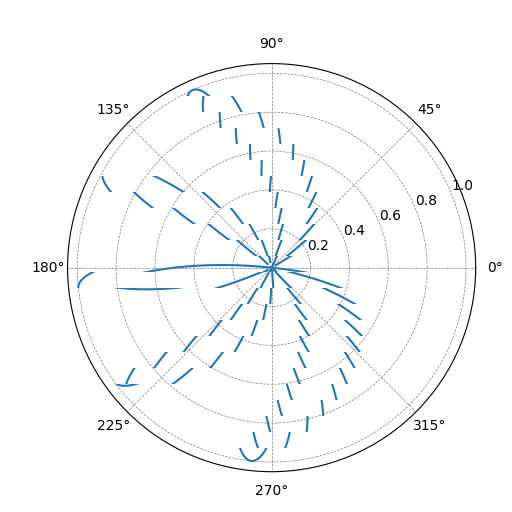
\includegraphics[scale=0.55]{images/shutter_effect.png}
    \\ \small Obraz 3. Obraz śmigła wygenerowany przez funkcje powyżej, $n = 5$.
\end{center}

\newpage
\section{Wnioski}
Zakłócenia ukazujące się w obrazie 3 wynikają z 
niespełnienia warunków twierdzenia o próbkowaniu. Obiekt
porusza się zbyt szybko, by macierz sensora zarejestrowała 
wszystkie piksele. Przykładowe sposoby na zniwelowanie 
tego efektu:
\vspace{0.25cm}
\begin{itemize}
    \item Unikanie ruchu podczas filmowania / trzymanie kamery 
    nieruchomo zminimalizuje zniekształcenia,
    \item Zwiększenie prędkości odczytu sensora, by była 
    większa od prędkości obracania się łopatek.
\end{itemize}

\vspace{0.25cm}
* Uniwersalną funkcją może ta ,którą użyliśmy w poprzednich zadaniach,
$f(x) = sin(nx + \frac{m\pi}{RPM})$, wystarczy zmieniać tylko
parametr $n$ w zależności od tego ile śmigieł chcemy. Przy większej 
ilości łopatek warto będzie, także zwiększyć wielkość generowanego obrazu.
\end{document}